\subsection{Creating an Assembly Duct Composed of Water}

First, create a new rectilinear core, and add a new duct to the assembly by following ~\ref{fig:Rect1}.

\begin{figure}[htb]
\begin{center}
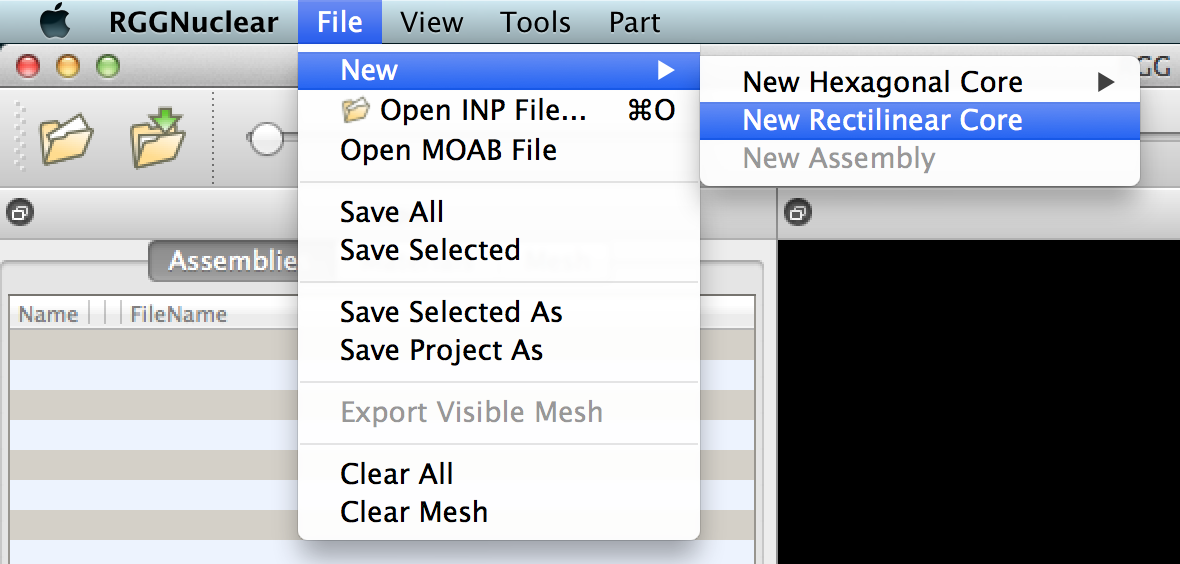
\includegraphics[width=0.5\linewidth]{Images/rect-1e1.png}
\caption{Select the option to create a new rectilinear assembly duct.}
\label{fig:Rect1}
\end{center}
\end{figure}

Next, right-click on the assembly and choose ``Create Duct''.

\begin{figure}[htb]
\begin{center}
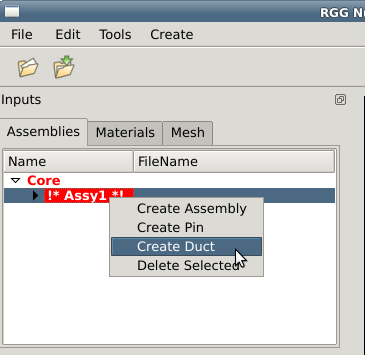
\includegraphics[width=0.5\linewidth]{Images/rect-2e1.png}
\caption{Create a new duct.}
\label{fig:Rect2}
\end{center}
\end{figure}

Tweak the dimensions of the duct, and choose ``water'' as its material.  The settings are shown in ~\ref{fig:Rect3}.

The result should look like ~\ref{fig:Rect4}.  Try manipulating the duct in the render window to verify its dimensions.

\begin{figure}
\centering
\begin{subfigure}{.5\textwidth}
  \centering
  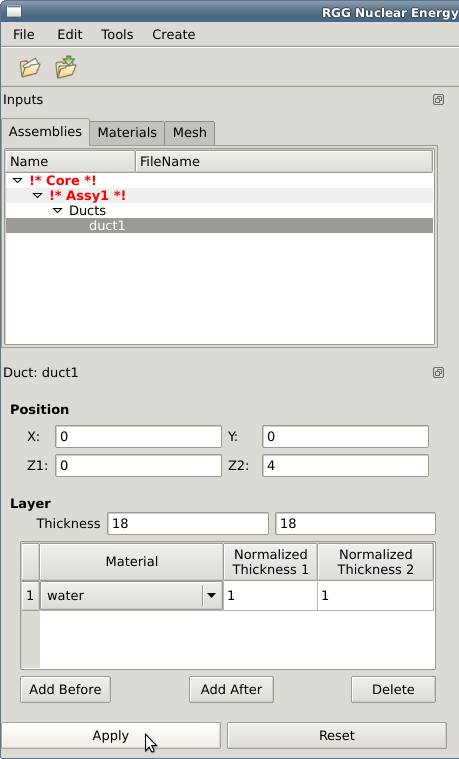
\includegraphics[width=0.7\linewidth]{Images/rect-3e1.png}
  \caption{Parameters for the duct.}
  \label{fig:Rect3}
\end{subfigure}%
\begin{subfigure}{.5\textwidth}
  \centering
  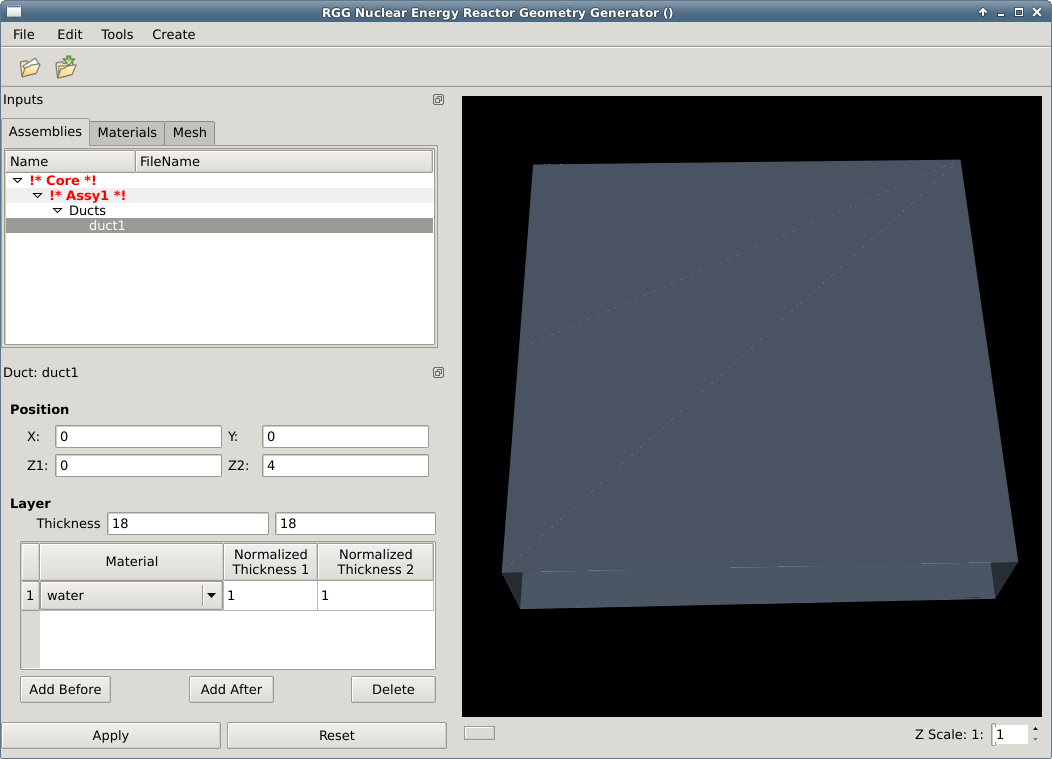
\includegraphics[width=0.9\linewidth]{Images/rect-4.png}
  \caption{The final product.}
  \label{fig:Rect4}
\end{subfigure}
\caption{Finished water duct.}
\label{fig:test}
\end{figure}

\clearpage

\subsection{Creating a Fuel Pin}

Right-click on the assembly and this time choose ``Create Pin''.

\subsubsection{Changing the Parameters}

Choose the dimensions of the pin to correspond to the dimensions of your duct.  In our case we have used a length of 4, corresponding to the height of the duct.

\begin{figure}[htb]
\begin{center}
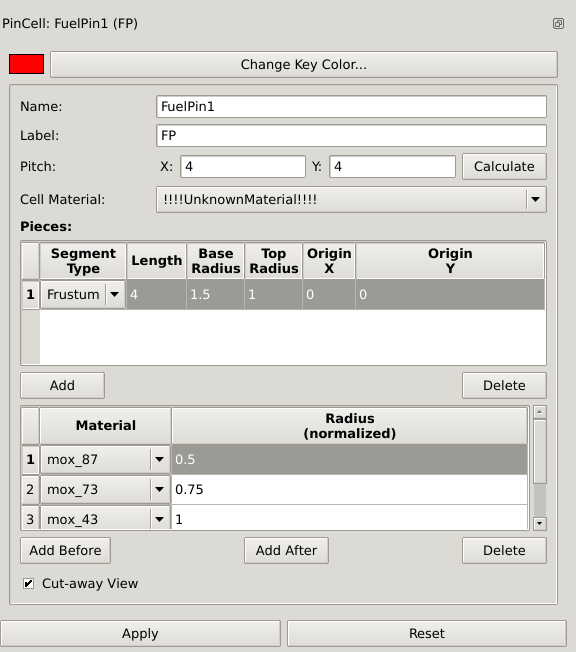
\includegraphics[width=0.4\linewidth]{Images/rect-5.png}
\caption{Fuel pin parameters.}
\label{fig:Rect5}
\end{center}
\end{figure}

Changing the key color and label is recommended, because later this will make the fuel pin more recognizeable while organizing the assembly.

\begin{wrapfigure}{r}{0.5\textwidth}
  \begin{center}
    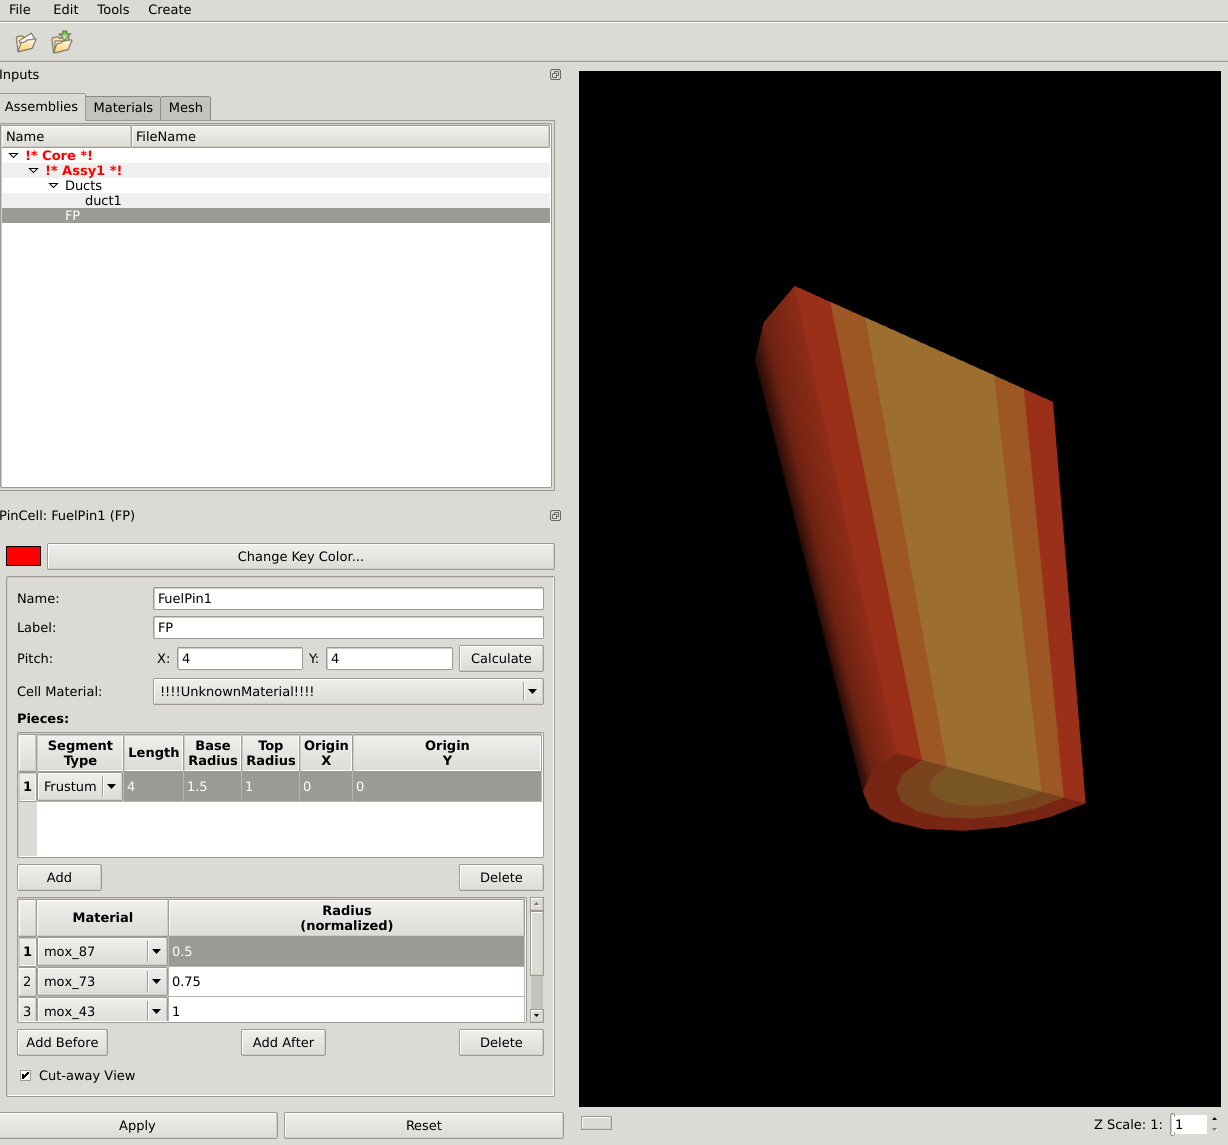
\includegraphics[width=0.48\textwidth]{Images/rect-6}
  \end{center}
  \caption{Final fuel pin product.}
  \label{fig:Rect6}
\end{wrapfigure}
Using the ``Add Before'' button, you can create a fuel pin with different layers of materials.  Refer to ~\ref{fig:Rect5} for the parameters used for our example, and ~\ref{fig:Rect6} to view the final product.

Note also the option to toggle the fuel pin's shape between a cylinder and a frustum.  The ``Cutaway view'' helps to view how the different materials are distributed within the fuel pin.

\subsection{Creating a Control Rod}
\begin{wrapfigure}{r}{0.5\textwidth}
  \begin{center}
    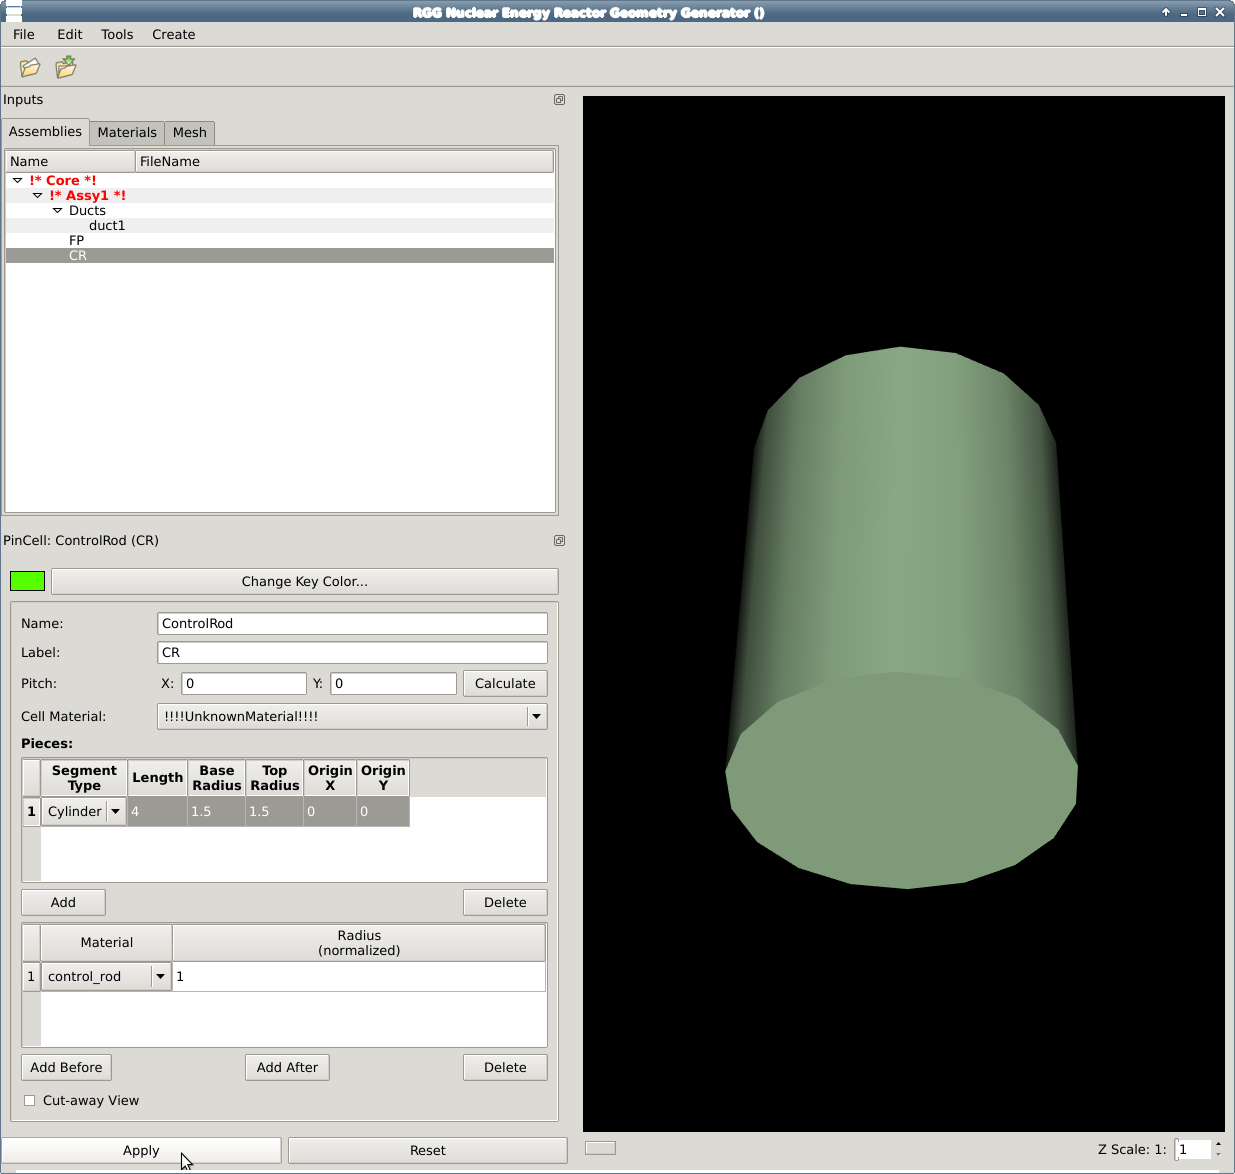
\includegraphics[width=0.48\textwidth]{Images/rect-7.png}
  \end{center}
  \caption{Final control product.}
  \label{fig:Rect7}
\end{wrapfigure}
Control rods are used to control nuclear fission. They are made out of materials which can easily absorb neutrons without undergoing fission themselves such as certain isotopes of boron, silver, or cadmium.

This is created using largely the same process as creating the fuel pin.  You can use the ``control rod'' material.  Once again, it's beneficial to change the key color to green.

Refer to ~\ref{fig:Rect7} for the final product.
\clearpage
\subsection{Adding Fuel Pins to the Assembly}

Now we want to add the pins we've created back to the assembly.  Click back on ``Assy 1'' in the assemblies view in order to see the assembly layout.  You should once again be able to see the water duct you created, and it should still be empty.  Compare your view with ~\ref{fig:Rect8}.

\begin{figure}[htb]
\begin{center}
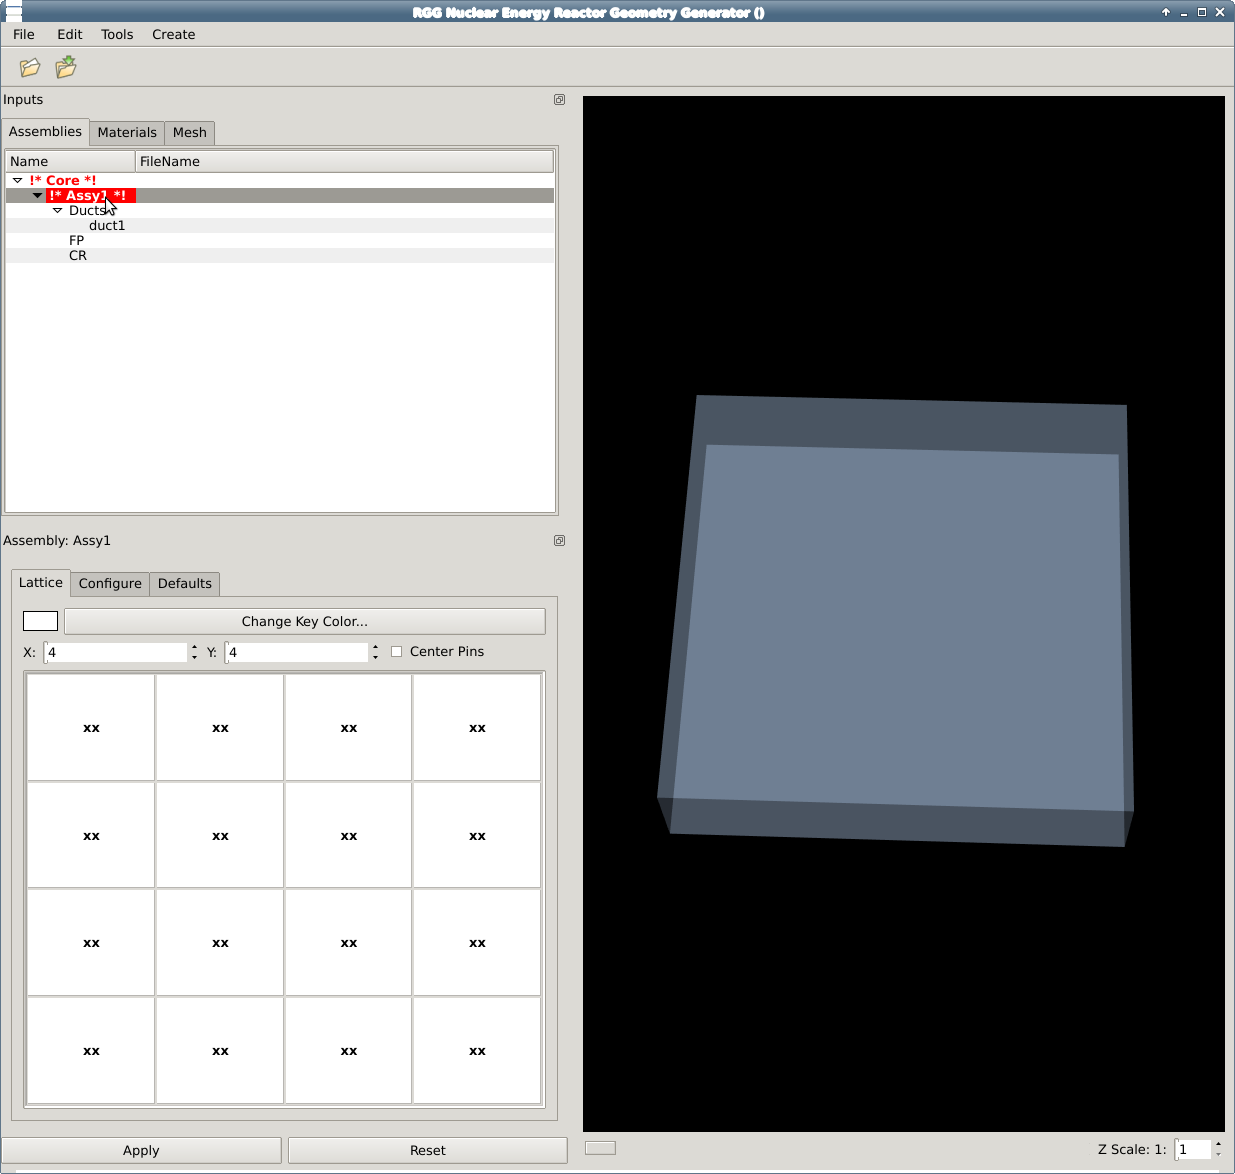
\includegraphics[width=0.4\linewidth]{Images/rect-8.png}
\caption{Empty duct in the assemblies view.}
\label{fig:Rect8}
\end{center}
\end{figure}

\begin{figure}[htb]
\begin{center}
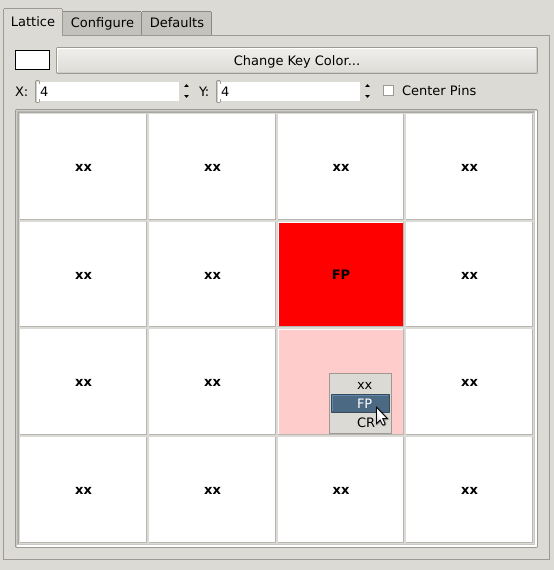
\includegraphics[width=0.4\linewidth]{Images/rect-9e1.png}
\caption{Right-click to organize the assembly.}
\label{fig:Rect9}
\end{center}
\end{figure}
Right click on each square and choose which pin to assign to it.  Alternatively, you can drag and drop pins already placed onto new squares.

In the end you should end up with something like ~\ref{fig:Rect10}.  If you find that the pins are placed in positions you didn't specify, go back to the pins and verify that the ``Pitch'' parameters are set to $X=4$ and $Y=4$ for each fuel pin and control rod.

Remember to click ``Apply'' in order to see your changes in the render window, or save them before navigating to another tab or pin.

\begin{figure}[htb]
\begin{center}
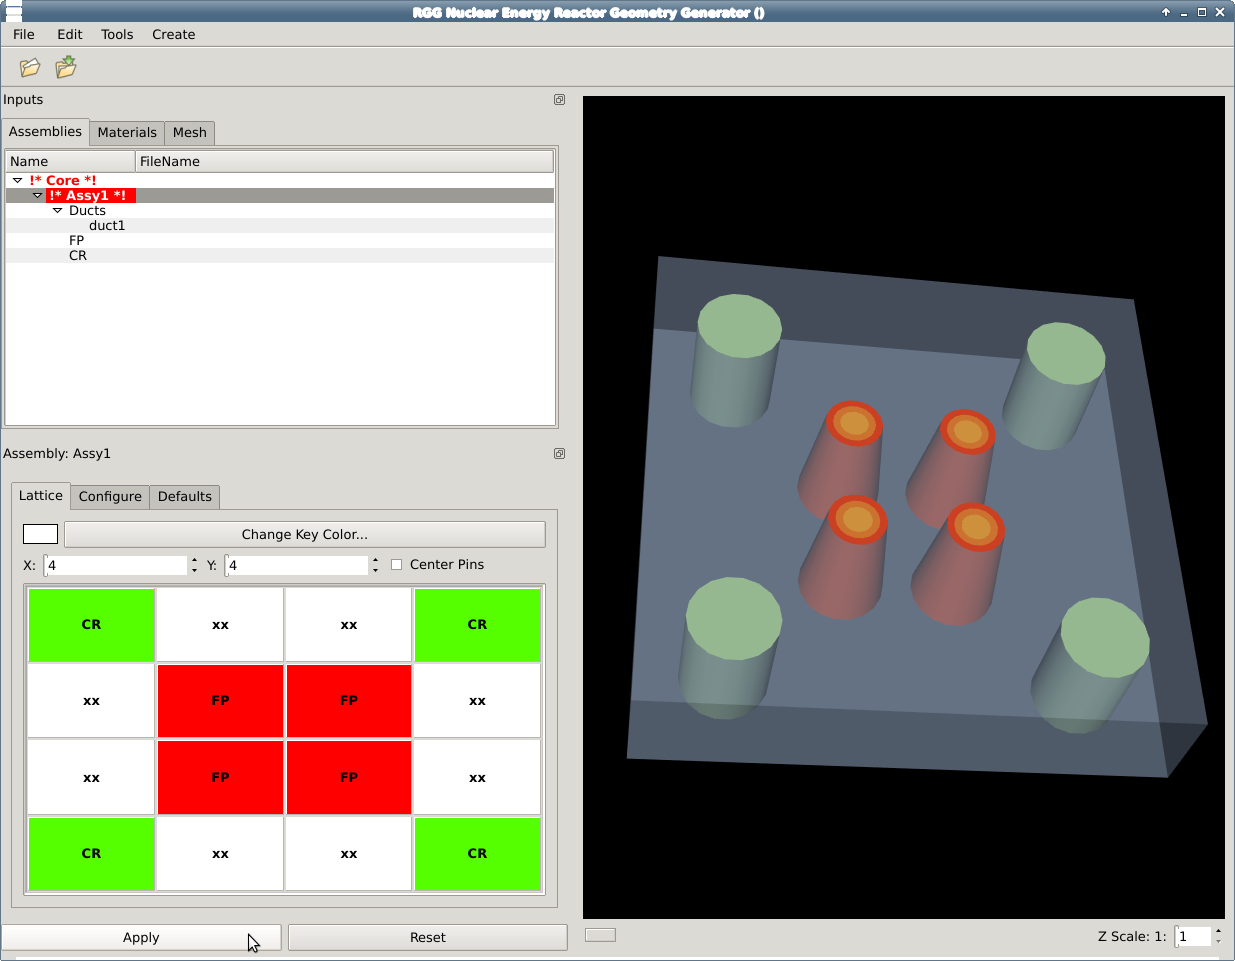
\includegraphics[width=0.7\linewidth]{Images/rect-10.png}
\caption{Final assembly.}
\label{fig:Rect10}
\end{center}
\end{figure}

